\newpage
\hypertarget{invertCard vis}{}
\subsection{Implementing invert}
\visHeader

\begin{itemize}

\vspace{0.5cm}

\item[$\blacktriangleright$] If you've completed all the work so far, you've got to be \emph{really} good at SDMs now. Model the simple story diagram
depicted in Fig.~\ref{ea:sdm_invertEmpty}.

\vspace{0.5cm}

\begin{figure}[htbp]
\begin{center}
  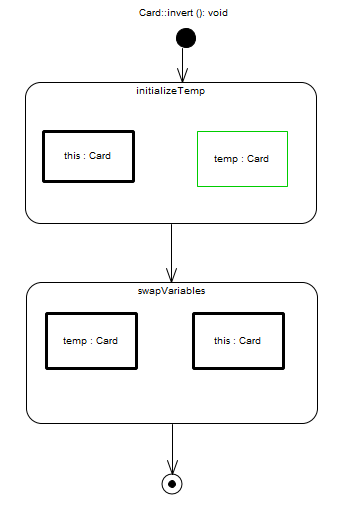
\includegraphics[width=0.6\textwidth]{ea_invertEmpty}
  \caption{Imperative control layer for inverting a card}  
  \label{ea:sdm_invertEmpty}
\end{center}
\end{figure}

\item[$\blacktriangleright$] Note that the binding operator on the first \texttt{temp} object variable is set to \texttt{create} (thus the green
border). This means that we actually \emph{create} a new object, and do not pattern match to an existing one in our model.

\item[$\blacktriangleright$] This activity will need four assignment constraints - two in \texttt{in\-it\-ia\-lize\-Temp} (to store the ``opposite'' values),
and two in \texttt{swapVariables} (to switch the values). Create your first assignment constraint by going to the created \texttt{temp} card and using the
`\texttt{:=}' operator to set the \texttt{temp.back} value to \texttt{this.face} (Fig.~\ref{ea:sdm_invertAssignment}).

\begin{figure}[htbp]
\begin{center}
  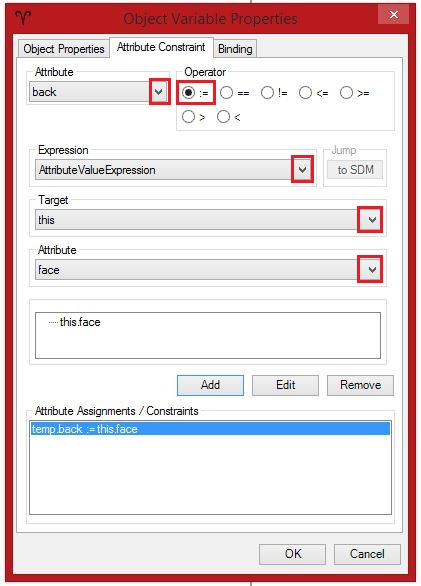
\includegraphics[width=0.7\textwidth]{ea_invertAttConstAssign}
  \caption{Store the \texttt{back} and \texttt{face} values of the card in \texttt{temp}}  
  \label{ea:sdm_invertAssignment}
\end{center}
\end{figure}

\clearpage

\vspace*{0.5cm}

\item[$\blacktriangleright$] Complete the SDM with the remaining constraints according to Fig.~\ref{ea:sdm_invertComplete} below.

\vspace{0.5cm}

\begin{figure}[htbp]
\begin{center}
  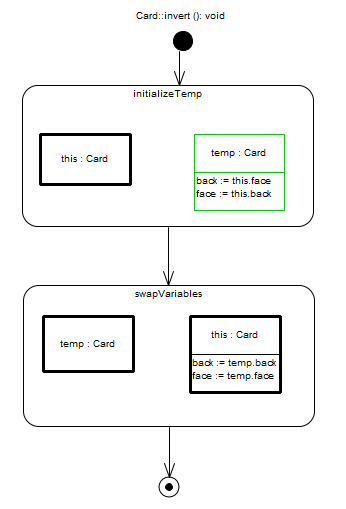
\includegraphics[width=0.7\textwidth]{ea_invertComplete}
  \caption{Swap back and face of the card}  
  \label{ea:sdm_invertComplete}
\end{center}
\end{figure}

\vspace{0.5cm}

\item[$\blacktriangleright$] Believe or not, that's it! Check out how this method is implemented in the textual syntax by reviewing
Fig.~\ref{eclipse:invertPatterns} in the next section. You don't \emph{have} to export and build to Eclipse, but it's always nice to confirm your work is error
free.

\jumpSingle{invert close} 

\end{itemize}
